\subsection{Paquete 2: Gestión de inmuebles, publicaciones y confianza}

    Las funcionalidades de este paquete cubren la búsqueda de alojamientos, las valoraciones entre usuarios y la administración de propiedades por parte de los propietarios. Para mantener una escala legible en los diagramas UML, el contenido se estructura en dos bloques: la búsqueda pública con reseñas, y la gestión física de inmuebles y anuncios.

\subsubsection{Exploración de alojamientos, recomendaciones y sistema de confianza}

    El primer bloque define la localización de habitaciones, la visualización en mapas y el intercambio de reseñas entre residentes. La figura \ref{fig:dcu_busqueda_resenas} muestra las relaciones entre actores y los ocho casos de uso del módulo (CU16 a CU23).

\begin{figure}[H]
    \centering
    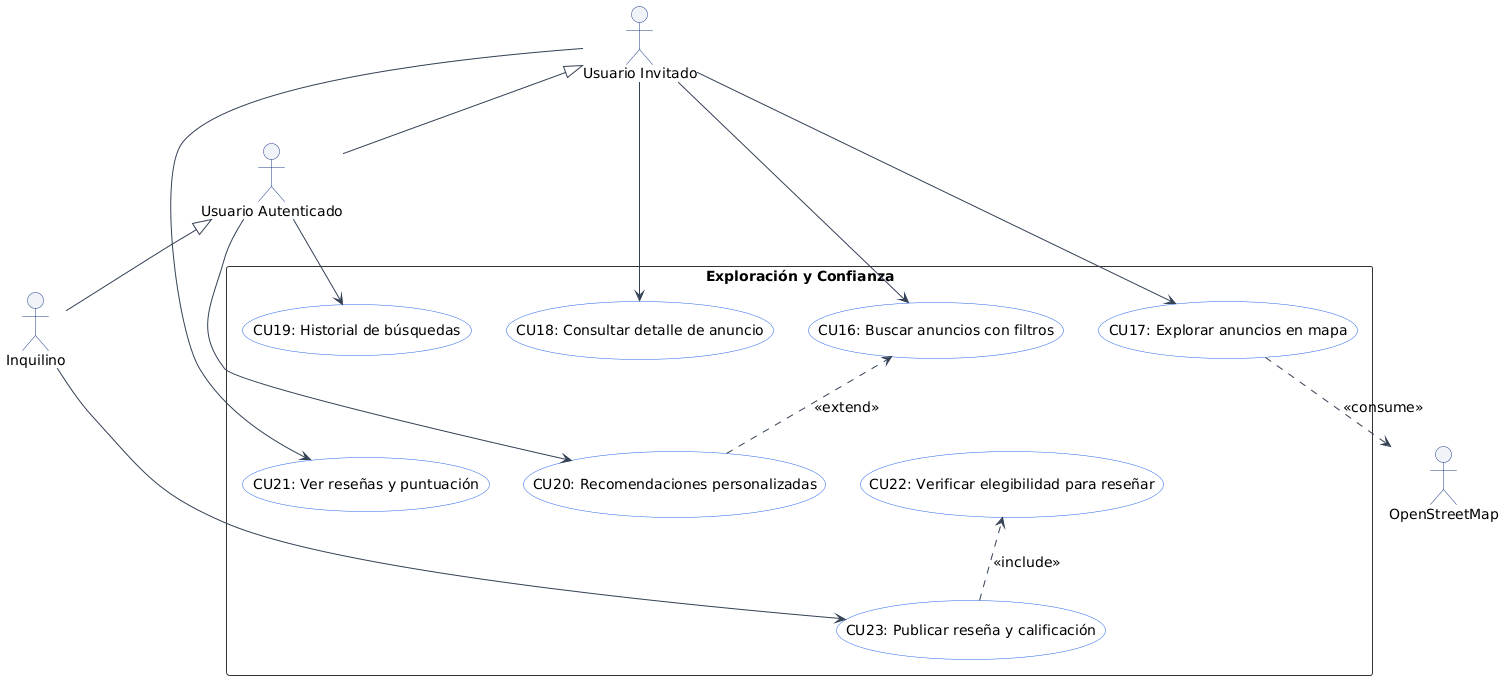
\includegraphics[width=0.88\textwidth]{AnalisisFuncional/img/dcu_busqueda_resenas.png}
    \caption{Diagrama de casos de uso de exploración, recomendaciones y reseñas}
    \label{fig:dcu_busqueda_resenas}
\end{figure}

    Las fichas de especificación funcional para este bloque comprenden desde CU16 hasta CU23:

\begin{table}[H]
\centering
\begin{tabular}{|p{3.1cm}|p{10.9cm}|}
\hline
\textbf{Caso de Uso} & \textbf{CU16: Buscar anuncios con filtros combinados} \\ \hline
\textbf{Actores} & Usuario Invitado, Usuario Autenticado \\ \hline
\textbf{Descripción} & Permite filtrar el catálogo de alojamientos según ciudad, rango de precio, tipo de habitación y servicios incluidos \\ \hline
\textbf{Precondiciones} & Que existan anuncios publicados y activos en la plataforma \\ \hline
\textbf{Flujo básico} & 
1. El usuario accede al explorador del catálogo e introduce los criterios de búsqueda. \newline
2. El sistema consulta la base de datos aplicando los filtros de forma acumulativa. \newline
3. El sistema devuelve los resultados paginados y actualiza la lista visual. \\ \hline
\end{tabular}
\caption{Especificación del caso de uso CU16.}
\label{tab:cu16}
\end{table}

\begin{table}[H]
\centering
\begin{tabular}{|p{3.1cm}|p{10.9cm}|}
\hline
\textbf{Caso de Uso} & \textbf{CU17: Explorar anuncios en mapa interactivo} \\ \hline
\textbf{Actores} & Usuario Invitado, Usuario Autenticado, OpenStreetMap / Nominatim \\ \hline
\textbf{Descripción} & Muestra los anuncios disponibles mediante marcadores geográficos sobre un mapa interactivo \\ \hline
\textbf{Precondiciones} & Disponer de conectividad con el servicio cartográfico \\ \hline
\textbf{Flujo básico} & 
1. El usuario activa la vista de mapa en el catálogo de alojamientos. \newline
2. El cliente solicita los marcadores comprendidos dentro del área geográfica visible. \newline
3. El sistema renderiza las posiciones y permite interactuar con las tarjetas emergentes. \\ \hline
\end{tabular}
\caption{Especificación del caso de uso CU17.}
\label{tab:cu17}
\end{table}

\begin{table}[H]
\centering
\begin{tabular}{|p{3.1cm}|p{10.9cm}|}
\hline
\textbf{Caso de Uso} & \textbf{CU18: Consultar detalle de anuncio y habitaciones} \\ \hline
\textbf{Actores} & Usuario Invitado, Usuario Autenticado \\ \hline
\textbf{Descripción} & Presenta la ficha completa de un anuncio, su galería gráfica, normas, fianza y habitaciones disponibles \\ \hline
\textbf{Precondiciones} & Que el anuncio seleccionado exista y se encuentre en estado visible \\ \hline
\textbf{Flujo básico} & 
1. El usuario pulsa sobre la tarjeta de un alojamiento desde la lista o el mapa. \newline
2. El sistema recupera los datos del inmueble, equipamiento, perfil del anfitrión y reseñas. \newline
3. La interfaz despliega la información organizada en pestañas de detalle. \\ \hline
\end{tabular}
\caption{Especificación del caso de uso CU18.}
\label{tab:cu18}
\end{table}

\begin{table}[H]
\centering
\begin{tabular}{|p{3.1cm}|p{10.9cm}|}
\hline
\textbf{Caso de Uso} & \textbf{CU19: Consultar historial de búsquedas} \\ \hline
\textbf{Actores} & Usuario Autenticado \\ \hline
\textbf{Descripción} & Muestra los términos, rangos de precios y ubicaciones consultadas recientemente \\ \hline
\textbf{Precondiciones} & Mantener una sesión activa con actividad previa registrada \\ \hline
\textbf{Flujo básico} & 
1. El usuario interactúa con la barra de búsqueda o el panel de filtros. \newline
2. El sistema recupera el registro cronológico de consultas previas del usuario. \newline
3. La interfaz presenta sugerencias directas basadas en las preferencias recientes. \\ \hline
\end{tabular}
\caption{Especificación del caso de uso CU19.}
\label{tab:cu19}
\end{table}

\begin{table}[H]
\centering
\begin{tabular}{|p{3.1cm}|p{10.9cm}|}
\hline
\textbf{Caso de Uso} & \textbf{CU20: Obtener recomendaciones personalizadas} \\ \hline
\textbf{Actores} & Usuario Autenticado \\ \hline
\textbf{Descripción} & Extiende la búsqueda de anuncios calculando sugerencias acordes al perfil y búsquedas previas \\ \hline
\textbf{Precondiciones} & Disponer de un historial de navegación con al menos una consulta registrada \\ \hline
\textbf{Flujo básico} & 
1. El usuario accede a la sección de recomendaciones en la pantalla de inicio. \newline
2. El motor de afinidad analiza las búsquedas guardadas y las características del perfil. \newline
3. El sistema ejecuta una búsqueda extendida y devuelve los alojamientos con mayor coincidencia. \\ \hline
\end{tabular}
\caption{Especificación del caso de uso CU20.}
\label{tab:cu20}
\end{table}

\begin{table}[H]
\centering
\begin{tabular}{|p{3.1cm}|p{10.9cm}|}
\hline
\textbf{Caso de Uso} & \textbf{CU21: Ver reseñas y puntuación media} \\ \hline
\textbf{Actores} & Usuario Invitado, Usuario Autenticado \\ \hline
\textbf{Descripción} & Consulta las opiniones, comentarios y calificaciones otorgadas a un alojamiento \\ \hline
\textbf{Precondiciones} & Que la publicación cuente con valoraciones registradas \\ \hline
\textbf{Flujo básico} & 
1. El usuario accede a la pestaña de opiniones dentro de la ficha de detalle. \newline
2. El sistema recupera las reseñas aprobadas y desglosa la media por categorías. \newline
3. La interfaz muestra los comentarios ordenados cronológicamente con la firma del autor. \\ \hline
\end{tabular}
\caption{Especificación del caso de uso CU21.}
\label{tab:cu21}
\end{table}

\begin{table}[H]
\centering
\begin{tabular}{|p{3.1cm}|p{10.9cm}|}
\hline
\textbf{Caso de Uso} & \textbf{CU22: Verificar elegibilidad para reseñar} \\ \hline
\textbf{Actores} & Inquilino \\ \hline
\textbf{Descripción} & Comprueba si el inquilino ha completado una estancia formalmente reservada en el inmueble \\ \hline
\textbf{Precondiciones} & Estar autenticado en el sistema \\ \hline
\textbf{Flujo básico} & 
1. El sistema intercepta el intento de emitir una valoración sobre un alojamiento. \newline
2. El backend audita el histórico de reservas confirmadas y finalizadas del usuario. \newline
3. El sistema comprueba que no exista una valoración previa emitida por la misma estancia. \newline
4. Si la comprobación es favorable, se autoriza la apertura del formulario de reseña. \\ \hline
\end{tabular}
\caption{Especificación del caso de uso CU22.}
\label{tab:cu22}
\end{table}

\begin{table}[H]
\centering
\begin{tabular}{|p{3.1cm}|p{10.9cm}|}
\hline
\textbf{Caso de Uso} & \textbf{CU23: Publicar reseña y calificación} \\ \hline
\textbf{Actores} & Inquilino \\ \hline
\textbf{Descripción} & Registra una valoración numérica de uno a cinco y un comentario descriptivo sobre la estancia \\ \hline
\textbf{Precondiciones} & Haber superado la verificación de elegibilidad previa \\ \hline
\textbf{Flujo básico} & 
1. El inquilino completa las puntuaciones desglosadas y redacta su opinión. \newline
2. Se ejecuta de forma obligatoria la verificación de elegibilidad. \newline
3. El sistema persiste la reseña en la base de datos y recalcula la media del alojamiento. \\ \hline
\end{tabular}
\caption{Especificación del caso de uso CU23.}
\label{tab:cu23}
\end{table}

\subsubsection{Gestión de inmuebles y ciclo de publicación del anfitrión}

    El segundo bloque abarca el registro de la vivienda física, su posicionamiento geográfico, la carga de fotos en Cloudinary y el control de publicación de las habitaciones. La figura \ref{fig:dcu_anfitrion_inmuebles} recoge los ocho casos de uso asociados (CU24 a CU31).

\begin{figure}[H]
    \centering
    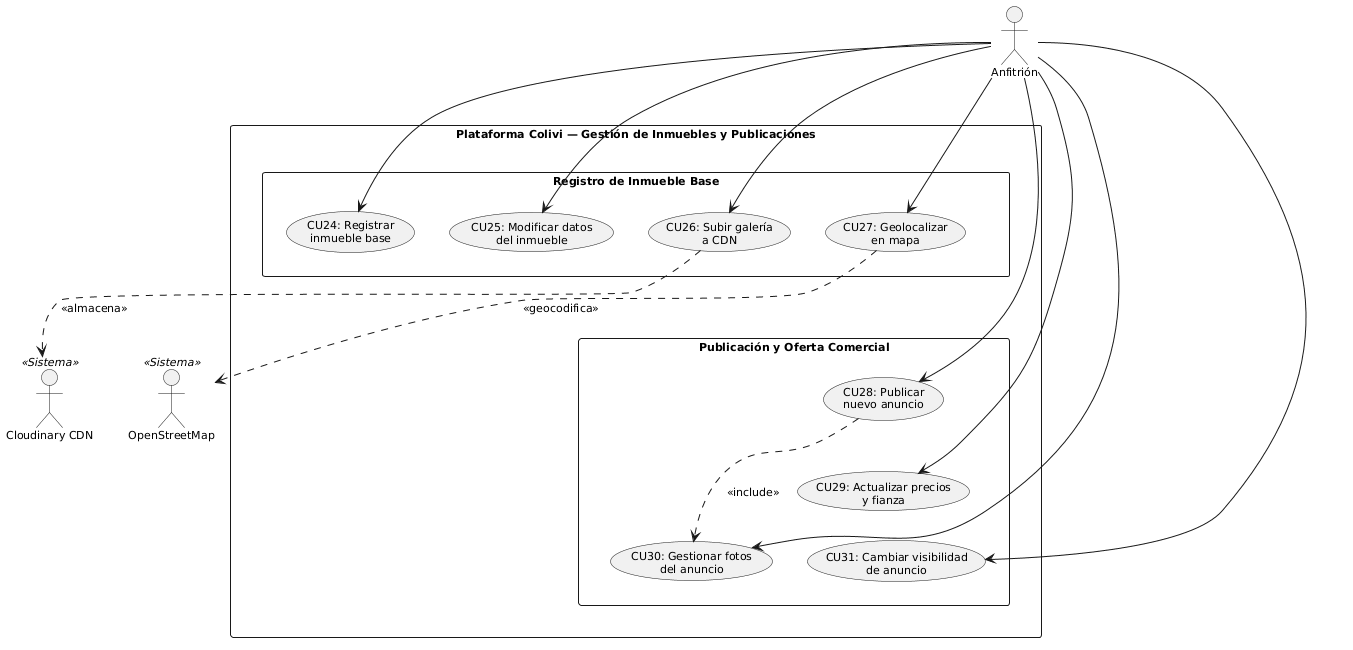
\includegraphics[width=0.88\textwidth]{AnalisisFuncional/img/dcu_anfitrion_inmuebles.png}
    \caption{Diagrama de casos de uso de gestión de inmuebles y publicaciones del anfitrión}
    \label{fig:dcu_anfitrion_inmuebles}
\end{figure}

    Las especificaciones funcionales de este ciclo se detallan desde CU24 hasta CU31:

\begin{table}[H]
\centering
\begin{tabular}{|p{3.1cm}|p{10.9cm}|}
\hline
\textbf{Caso de Uso} & \textbf{CU24: Registrar inmueble base} \\ \hline
\textbf{Actores} & Anfitrión \\ \hline
\textbf{Descripción} & Da de alta la estructura física de una vivienda definiendo superficie, estancias comunes y servicios \\ \hline
\textbf{Precondiciones} & Estar autenticado con perfil de anfitrión \\ \hline
\textbf{Flujo básico} & 
1. El anfitrión accede al asistente de registro de propiedades. \newline
2. El anfitrión especifica la dirección, metros cuadrados, número de habitaciones y zonas comunes. \newline
3. El sistema valida la integridad de los datos y almacena el registro del inmueble base. \\ \hline
\end{tabular}
\caption{Especificación del caso de uso CU24.}
\label{tab:cu24}
\end{table}

\begin{table}[H]
\centering
\begin{tabular}{|p{3.1cm}|p{10.9cm}|}
\hline
\textbf{Caso de Uso} & \textbf{CU25: Modificar datos del inmueble base} \\ \hline
\textbf{Actores} & Anfitrión \\ \hline
\textbf{Descripción} & Permite actualizar la descripción o los equipamientos compartidos de una propiedad \\ \hline
\textbf{Precondiciones} & Ser el titular propietario del inmueble \\ \hline
\textbf{Flujo básico} & 
1. El anfitrión accede al panel de gestión de sus propiedades y selecciona la vivienda. \newline
2. El anfitrión modifica las características físicas o los servicios disponibles. \newline
3. El backend verifica la titularidad y persiste los cambios actualizados. \\ \hline
\end{tabular}
\caption{Especificación del caso de uso CU25.}
\label{tab:cu25}
\end{table}

\begin{table}[H]
\centering
\begin{tabular}{|p{3.1cm}|p{10.9cm}|}
\hline
\textbf{Caso de Uso} & \textbf{CU26: Subir galería fotográfica a CDN} \\ \hline
\textbf{Actores} & Anfitrión, Cloudinary CDN \\ \hline
\textbf{Descripción} & Transfiere un conjunto de imágenes para asociarlas a la ficha del inmueble \\ \hline
\textbf{Precondiciones} & Archivos en formato gráfico admitido que no superen el límite de tamaño establecido \\ \hline
\textbf{Flujo básico} & 
1. El anfitrión selecciona una o varias imágenes desde su explorador local. \newline
2. El cliente transfiere los archivos binarios hacia el servicio de almacenamiento seguro. \newline
3. Cloudinary optimiza y custodia los recursos, retornando los enlaces HTTPS persistentes. \newline
4. El backend almacena las referencias de las imágenes vinculándolas al inmueble. \\ \hline
\end{tabular}
\caption{Especificación del caso de uso CU26.}
\label{tab:cu26}
\end{table}

\begin{table}[H]
\centering
\begin{tabular}{|p{3.1cm}|p{10.9cm}|}
\hline
\textbf{Caso de Uso} & \textbf{CU27: Geolocalizar dirección en mapa} \\ \hline
\textbf{Actores} & Anfitrión, OpenStreetMap / Nominatim \\ \hline
\textbf{Descripción} & Convierte la dirección postal introducida en coordenadas geográficas de latitud y longitud \\ \hline
\textbf{Precondiciones} & Introducir una dirección válida con calle, número, código postal y ciudad \\ \hline
\textbf{Flujo básico} & 
1. El anfitrión escribe la dirección postal durante el alta o edición del inmueble. \newline
2. El cliente remite la consulta al servicio de geocodificación de OpenStreetMap. \newline
3. El servicio devuelve las coordenadas geográficas correspondientes. \newline
4. El sistema posiciona el marcador en el mapa y almacena los valores espaciales. \\ \hline
\end{tabular}
\caption{Especificación del caso de uso CU27.}
\label{tab:cu27}
\end{table}

\begin{table}[H]
\centering
\begin{tabular}{|p{3.1cm}|p{10.9cm}|}
\hline
\textbf{Caso de Uso} & \textbf{CU28: Publicar nuevo anuncio} \\ \hline
\textbf{Actores} & Anfitrión \\ \hline
\textbf{Descripción} & Genera una oferta comercial en el catálogo vinculada a una habitación o al piso completo \\ \hline
\textbf{Precondiciones} & Disponer de un inmueble base registrado con al menos una fotografía \\ \hline
\textbf{Flujo básico} & 
1. El anfitrión pulsa la opción de crear publicación y selecciona el inmueble asociado. \newline
2. El anfitrión fija el título, descripción comercial, renta mensual, fianza y fechas de disponibilidad. \newline
3. Se invoca de forma obligatoria el caso de uso de gestión de fotografías del anuncio. \newline
4. El sistema valida las condiciones económicas y publica la oferta en el catálogo. \\ \hline
\end{tabular}
\caption{Especificación del caso de uso CU28.}
\label{tab:cu28}
\end{table}

\begin{table}[H]
\centering
\begin{tabular}{|p{3.1cm}|p{10.9cm}|}
\hline
\textbf{Caso de Uso} & \textbf{CU29: Actualizar precios, depósito y condiciones} \\ \hline
\textbf{Actores} & Anfitrión \\ \hline
\textbf{Descripción} & Permite reajustar los importes de alquiler, fianza requerida o normas de estancia \\ \hline
\textbf{Precondiciones} & Ser titular del anuncio publicado \\ \hline
\textbf{Flujo básico} & 
1. El anfitrión selecciona el anuncio y abre el formulario de condiciones contractuales. \newline
2. El anfitrión modifica la renta o la fianza y confirma los cambios. \newline
3. El sistema valida que los nuevos importes sean valores numéricos positivos. \newline
4. El backend actualiza la oferta sin alterar las reservas previamente confirmadas. \\ \hline
\end{tabular}
\caption{Especificación del caso de uso CU29.}
\label{tab:cu29}
\end{table}

\begin{table}[H]
\centering
\begin{tabular}{|p{3.1cm}|p{10.9cm}|}
\hline
\textbf{Caso de Uso} & \textbf{CU30: Seleccionar y ordenar imágenes para el anuncio} \\ \hline
\textbf{Actores} & Anfitrión \\ \hline
\textbf{Descripción} & Organiza la galería de fotografías del anuncio y define la imagen de portada principal \\ \hline
\textbf{Precondiciones} & Que el inmueble asociado disponga de imágenes cargadas en el servidor \\ \hline
\textbf{Flujo básico} & 
1. El anfitrión visualiza la cuadrícula de fotografías asignadas a la propiedad. \newline
2. El anfitrión reordena las imágenes y marca la que actuará como cabecera. \newline
3. El sistema guarda la secuencia de ordenamiento para su renderizado en catálogo. \\ \hline
\end{tabular}
\caption{Especificación del caso de uso CU30.}
\label{tab:cu30}
\end{table}

\begin{table}[H]
\centering
\begin{tabular}{|p{3.1cm}|p{10.9cm}|}
\hline
\textbf{Caso de Uso} & \textbf{CU31: Cambiar visibilidad de anuncio} \\ \hline
\textbf{Actores} & Anfitrión \\ \hline
\textbf{Descripción} & Conmuta el estado de una publicación entre disponible, pausada o archivada \\ \hline
\textbf{Precondiciones} & Ser el propietario del anuncio \\ \hline
\textbf{Flujo básico} & 
1. El anfitrión selecciona la acción de cambio de estado en el panel de control. \newline
2. El sistema actualiza el atributo de visibilidad de la publicación. \newline
3. El catálogo omite o incluye el anuncio en los filtros públicos de forma inmediata. \\ \hline
\end{tabular}
\caption{Especificación del caso de uso CU31.}
\label{tab:cu31}
\end{table}